


\begin{tcolorbox}[colback=blue!5!white,colframe=blue!75!black,title=Túnel de viento]
Es una herramienta que puede tener dos fines, ya sea para uso recreativo o para propósito científico.
Como uso científico se utiliza para observar los efectos del movimiento de aire alrededor de objetos sólidos, como también para la calibración de anemómetros, entre otros.
\end{tcolorbox}


\subsection{Clasificación}
Los túneles de viento se pueden clasificar en túneles abiertos o cerrados y a su vez pueden ser verticales u horizontales (Figuras: \ref{fig:abierto} y \ref{fig:tunelRec})


\begin{figure}[htbp]
    \centering
    \subfigure[Túnel tipo cerrado]{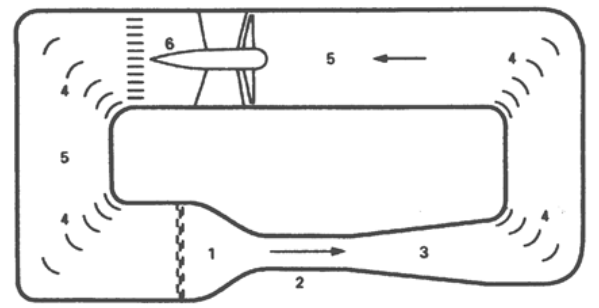
\includegraphics[width=60mm]{tunel_cerrado.png}}
    \subfigure[Túnel tipo abierto]{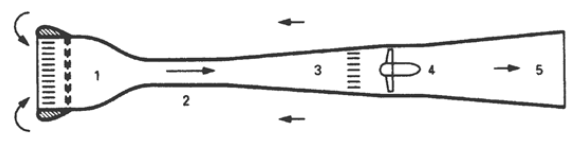
\includegraphics[width=80mm]{tunel_abierto.png}}
    \caption{Clasificación túneles} \label{fig:abierto}
    \end{figure}

\begin{figure}[htb]
	\centering
	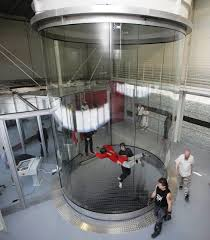
\includegraphics[scale=0.8]{tvert1.jpg}
	\captionof{figure}{Tunel vertical de uso recreativo}
	\label{fig:tunelRec}
\end{figure}

\subsection{Túnel UNPSJB}

\subsubsection{Historia}
\cite{tunelweb}	El túnel aerodinámico del Laboratorio de Mecánica de Fluidos (\textbf{LMF}) de la Facultad de Ingeniería de la Universidad Nacional de la Patagonia San Juan Bosco (\textbf{UNPSJB}) es un circuito abierto (tipo Eiffel) con cámara de ensayos cerrada. Puede clasificarse como un túnel “pequeño de baja velocidad”, con una longitud total de 11 $m$, una velocidad máxima de 18 $m/s$ y una cámara de ensayos con un área de 0,8 $m^2$.
	
	\begin{figure}[htb]
		\centering
		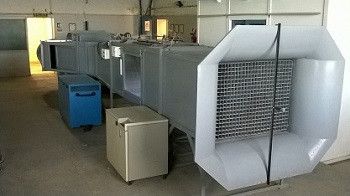
\includegraphics[scale=0.9]{tunel_unpsjb.JPG}
		\captionof{figure}{Tunel UNPSJB}
		\label{fig:tunelUni}
	\end{figure}
	
	La entrada del túnel cuenta con canalizadores, comúnmente denominados "panal de abejas", que favorecen la formación de un flujo uniforme y homogéneo.
	
	La cámara de ensayos es vidriada para poder observar con claridad el flujo y está incorporada en un módulo extraíble del túnel, lo cual permite fácil acceso para el armado de los distintos objetos a ensayar.
	
	Los distintos ensayos que se realizan en el túnel son:
	\begin{itemize}
		\item  Determinación de coeficientes de resistencia y sustentación de distintos cuerpos y perfiles aerodinámicos. 
		\item Determinación de distribución de presiones a través de diferentes objetos como perfiles aerodinámicos, edificios, puentes, automóviles, etc.
		\item Visualización con humo del flujo a través de distintos obstáculos.
		\item Estudio del comportamiento dinámico de generadores eólicos. 
		\item Calibración de anemómetros.
	\end{itemize}

	\subsubsection{Motor y Variador de velocidad}
		\begin{tcolorbox}[colback=blue!5!white,colframe=blue!75!black,title=Variador de velocidad]
			Es utilizado para controlar la velocidad de giro de un motor. Para regular las revoluciones, se debe tener en cuenta las características del motor, ya que este tiene  una  curva  propia  de  funcionamiento. 
			Un variador de velocidad es capaz de controlar la aceleración, frenado, torque, generar operaciones que mejoran la eficiencia energética y brindar seguridad.\end{tcolorbox}	

El motor utilizado para accionar el ventilador del túnel es del tipo de inducción de rotor bobinado, de 30kW de potencia, Marca \textbf{AEG}\cite{barila1993desarrollo}. Desde el año 2020, el laboratorio de Fluidos cuenta con un variador de velocidad de la marca \textbf{Long Shenq} modelo \textbf{LS650-4045} de 45kW trifásico \cite{LS650}.
 
Al utilizar este variador, la frecuencia puede ser controlada de forma manual por su panel frontal y/o por entradas tanto de corriente o tensión, las mismas se pueden configurar para el rango máximo de que podría ser de 0 a 300Hz en ambos sentidos, pero por razones constructivas del motor se utiliza en el rango de 13Hz a 53Hz en un sentido. Al ser un motor antiguo, de la década de 1920, no posee rodamientos sino cojinetes, y estos necesitan funcionar en rangos de aceleración y velocidades acotados, para evitar trabajar sin la necesaria película lubricante que evita el contacto directo entre los cojinetes y el eje de la máquina.


\begin{figure}[htb]
	\centering
	\subfigure[Motor y ventilador durante la construcción del túnel]{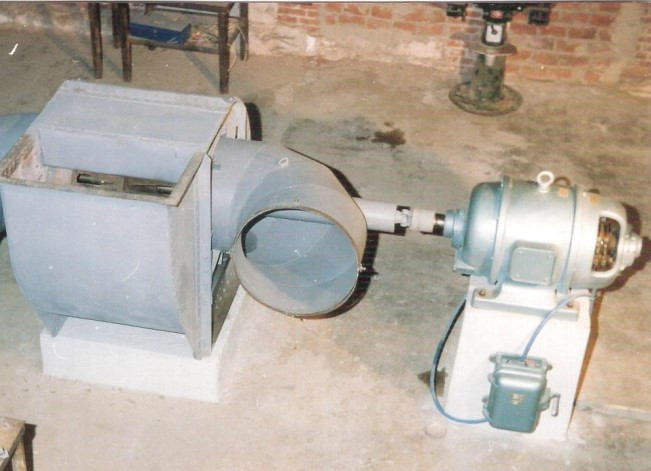
\includegraphics[height=7cm]{motor.jpg}}\label{fig:motorr}
	\hfill
	\subfigure[Variador de velocidad LS650]{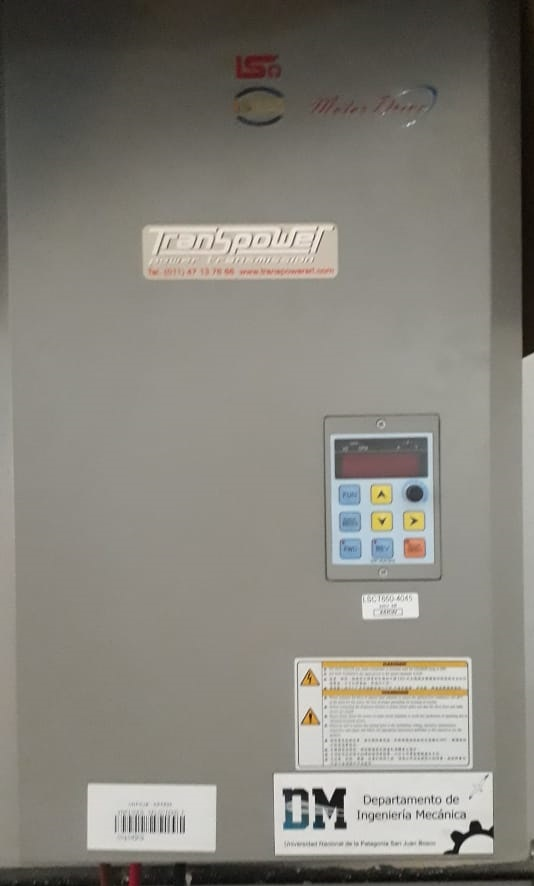
\includegraphics[height=7cm]{LS650.jpg}}\label{fig:LS650}
	\caption{Motor y variador de velocidad} 
	
\end{figure}



		
	\subsubsection{Instrumentación}
	Los instrumentos utilizados en las mediciones del túnel para la contrastación de anemómetros  están calibrados y certificados por el \textbf{INTI} (Instituto Nacional Tecnología Industrial).
\begin{itemize}
	\item \textbf{Micromanovacuómetro }
		\subitem Instrumento utilizado para medir la diferencia de presión.
		
		\textit{Marca: Alnor. Modelo: 560. Número de serie: 56057034.} 
	\item \textbf{Instrumento multifunción}
	\subitem  Utilizado para medir la temperatura, humedad y presión atmosférica. Este mismo elemento puede ser utilizado para medir la velocidad del aire.
	
	\textit{Tipo de instrumento: Termómetro electrónico. Sonda de hilo caliente para TESTO 435.  Modelo: Testo 435-2. Sonda
	número: 0635 1025. \\ Tipo de instrumento: Anemómetro electrónico. Modelo: Testo 435-2. Sonda número: 0635 1025.}
	
	
\end{itemize}	   		
		
\begin{figure}[htbp]
	\centering
	\subfigure[AXD 650]{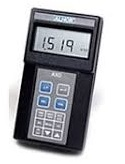
\includegraphics[width=40mm]{axd.jpg}}
	\subfigure[Testo 435]{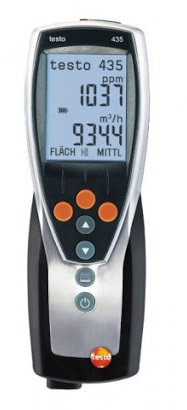
\includegraphics[scale=0.5]{testo.jpg}}
	\caption{Instrumentación calibrada} \label{fig:instr}
\end{figure}		
		
		
		\newpage